\section{Iterating the crossing bound}\label{sec:recursion}

Theorem~\ref{thm:seed} asks for $N$ prescribed physical intervals, each of
which costs at least $RN^{K-1}$ interior breaks to cross. We build this
cost inductively. Inside one episode, Lemma~\ref{lem:episode} identifies
$q_*$ disjoint portions of a crossing. Each either pays the crossing cost
of a system already built or traverses a designated physical overlap.
We place another episode inside every such overlap. At the last depth
of this nesting, a convex coordinate bound charges every traversal of
the overlap, including a return through the same interval.

\subsection{Forcing breaks at marked times}
Let $a_1,\ldots,a_s$ be distinct times and set
\[
                         f(x)=\sum_{k=1}^s\max\{0,x-a_k\}.
\]
This convex piecewise affine function has a strict change of slope at
each mark. On any signature $T$, take $J+1$ disjoint copies of the
one-request-per-node program from Section~\ref{sec:framework}. Impose
$z_i\ge f(x)$ on each of their coordinates, using one affine row per
piece of $f$. Call the resulting system a \emph{tracer}. We can add it
to another system on $T$ by giving it fresh coordinates and taking the
union of their programs, so both systems have the same physical time $x$.

Each copy must supply a usable coordinate. If all usable tracer
coordinates strictly exceeded $f(x)$, their independent coordinate
directions would lie in the kernel of the tight rows on the usable set.
Its dimension would then be at least $J+1$, contrary to
Definition~\ref{def:admissible}. Hence at every admissible point some
tracer coordinate attains its floor.

An affine segment of an admissible path cannot pass from $x<a_k$ to
$x>a_k$. At its interior point with $x=a_k$, some affine tracer row
is tight. Its slack is affine and nonnegative on the segment, so it must
vanish throughout. The affine right-hand side of that row lies strictly
below $f$ on at least one side of $a_k$, contrary to the coordinate
floor. The same argument applies in the reverse direction.

More generally, consider a crossing of an interval containing several
marks in its interior. Choose a disjoint small closed interval around
each mark. Orient the crossing toward the upper endpoint. For each
small interval take the last visit to its lower endpoint before the
first visit to its upper endpoint. This gives a traversal inside that
interval. The upper endpoint of one interval must be visited before
the lower endpoint of the next can be reached, so the chosen traversals
have disjoint parameter interiors. Each traversal contains a break:
without one it would be a single affine segment through the mark.
The same marks can impose these costs again on a later traversal
(Figure~\ref{fig:return-traversals}).

\begin{figure}[tbp]
\centering
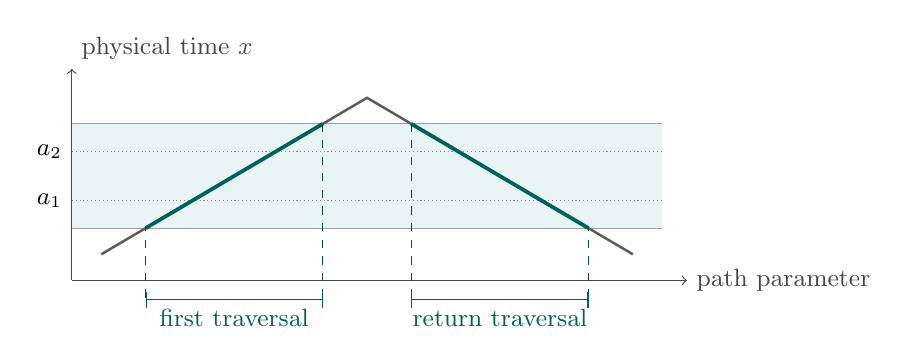
\begin{tikzpicture}[x=1.25cm,y=0.92cm,font=\small]
  \fill[teal!9] (0,0.72) rectangle (6.0,2.16);
  \draw[black!38] (0,0.72)--(6,0.72) (0,2.16)--(6,2.16);
  \foreach \y/\lab in {1.1/{a_1},1.78/{a_2}} {
    \draw[black!46,densely dotted] (0,\y)--(6,\y);
    \node[left] at (0,\y) {$\lab$};
  }
  \draw[->,black!72] (0,0)--(6.25,0) node[right] {path parameter};
  \draw[->,black!72] (0,0)--(0,2.92) node[above right] {physical time $x$};
  \draw[black!64,line width=.9pt] (.3,.36)--(3,2.52)--(5.7,.36);
  \draw[teal!75!black,line width=1.35pt] (.75,.72)--(2.55,2.16);
  \draw[teal!75!black,line width=1.35pt] (3.45,2.16)--(5.25,.72);
  \foreach \x/\y in {.75/.72,2.55/2.16,3.45/2.16,5.25/.72}
    \draw[teal!60!black,dashed] (\x,-.24)--(\x,\y);
  \draw[|-|,teal!75!black] (.75,-.27)--(2.55,-.27)
    node[midway,below] {first traversal};
  \draw[|-|,teal!75!black] (3.45,-.27)--(5.25,-.27)
    node[midway,below] {return traversal};
\end{tikzpicture}
\caption{Two visits to the same physical interval (shaded) occupy disjoint
parts of the path parameter. Each visit incurs a distinct interior break
for each tracer mark $a_1,a_2$. Only the time projection is drawn. A
break in a tracer coordinate need not be visible in that projection.}
\label{fig:return-traversals}
\end{figure}


\subsection{Nested episodes}
There are two depths in the construction. At level $j$, the clock and
resource inputs are systems from level $j-1$. Within a single level we
nest episodes in physical overlaps to depth $g_*$. This second depth
ensures that continuing through overlaps without taking an inner crossing
ultimately incurs just as many breaks.

Fix $K\ge2$ and $0<\eta<1$. For $N=L^h$, where the scheduler base $L$
will be fixed below, set
\[
  e=\frac{\eta}{200K},\qquad
  g_*=\lceil 2K/e\rceil,\qquad q_*=\lceil N^e\rceil .
\]
At each level the number $B_j$ of buckets must exceed four times the
label count $V$ times the dimension of the resource input. We allow
successively larger bucket counts by setting
\[
 b_K=\frac{e}{10g_*},\qquad b_{j-1}=\frac{b_j}{10g_*}\quad(3\le j\le K),
 \qquad B_j=\lceil N^{b_j}\rceil\quad(2\le j\le K).
\]
Set $J=1+\lfloor N^{b_2/8}\rfloor$. The integer multiplier $R\ge1$ controls
the number of marks and may be chosen independently of these parameters.

Write $Q_j(T)$ for a level-$j$ system on the signature $T$. At the top,
$T$ has one node. A level-$j$ driver on $T$ uses $Q_{j-1}(T)$ for its
clocks and $Q_{j-1}(T^+)$ for its resources. Since
Theorem~\ref{thm:scheduler} determines $T^+$ from $T$ before the client
program is chosen, all needed signatures are specified by descending
from the top. We now construct the systems in the opposite order.

At level one take a tracer with $RN$ distinct marked times in $(0,1)$.
At level $j\ge2$, every driver uses $B_j$ buckets and $q_*$ triples of
work windows. Label each overlap by its bucket and by its early or late
phase, giving the same alphabet of $2B_j$ labels in each episode. A word
in this alphabet records the successive overlaps in which an episode
is nested. Use one driver per word of length less than $g_*$.

The empty word indexes the driver with the $N$ prescribed disjoint
episodes in $(0,1)$. Once the driver for word $v$ is built, locate the
$i$th episode of the driver for $va$ strictly inside overlap $a$ of
the $i$th episode for $v$, for every $i$. Thus a child driver serves
all $N$ parent episodes. For $|v|=g_*-1$, choose $R$ distinct interior
times in each of its overlaps and put all these marks in one tracer.
The drivers and the tracer share $x$ and have separate coordinates.
Join their programs at $T$. This is $Q_j(T)$.

A viable set for the joined program restricts to a viable set on each
component. At fixed $x$ the tight coordinate matrix is block diagonal,
so its nullity on the usable coordinates of any component is at most
that of the whole matrix. Thus an admissible point projects to an
admissible point of each driver and of the tracer. In particular, every
viable set has more than $J$ coordinates, as required when $Q_j(T)$
itself becomes a driver input. The coordinate count below verifies
the bucket inequality at each level.

\begin{proposition}[Cost of a nested crossing]\label{prop:iterated-crossing}
Let $D_j=4^{1-j}RN^jq_*^{j-1}$. For all sufficiently large $N$, all
integers $R\ge1$, and all the signatures at level $1\le j\le K$, every segmentation
of an admissible crossing of $[0,1]$ in $Q_j(T)$ has at least $D_j$
segments. At levels $j\ge2$ every segmentation of an admissible traversal
of one empty-word episode has at least $D_j/N$ breaks in its parameter
interior. Both statements hold in either orientation.
\end{proposition}
\begin{proof}
The $RN$ marked times give the assertion for $j=1$. At level $j\ge2$ put
$A=D_{j-1}/2-1$ and fix a segmentation of the traversal. In any episode,
Lemma~\ref{lem:episode} supplies $q_*$ subpaths with disjoint parameter
interiors. Each either contains $A$ or more interior breaks or traverses
a designated overlap. In the latter case trim to the episode placed
inside that overlap. If this is a terminal overlap, use its $R$ tracer
marks instead. The segmentation induced by trimming has only original
breaks in its interior: the new endpoints never enter the count. This
remains true when two subpaths traverse the same physical overlap.

Let $E_t$ denote the lower bound obtained when $t$ driver levels remain
in this episode, counting the current driver. For a terminal overlap the
bound is $E_0=R$. Since a child charge is internal to its parent subpath,
the disjoint subpaths give the recurrence
\[
 E_t=q_*\min\{A,E_{t-1}\}
       =\min\{q_* A,Rq_*^t\}\qquad(t\ge1),
\]
where the second equality follows by induction. At the empty word
$t=g_*$. For large $N$ we have $D_{j-1}\ge4$, so $q_* A\ge
q_*D_{j-1}/4$. Also $q_*^{g_*}\ge N^{2K}\ge N^{j-1}q_*^{j-1}$
for $j\le K$ and sufficiently large $N$. Thus
\[
                     E_{g_*}\ge q_*D_{j-1}/4=D_j/N .
\]
Every full crossing has a traversal of each of the $N$ empty-word
episodes. Taking the first visit to the far endpoint and the last visit
to the near endpoint before it gives these traversals in order,
with disjoint parameter interiors. Hence the full crossing incurs
at least $D_j$ interior breaks and, in particular, at least $D_j$
segments.
\end{proof}

\subsection{Dimension and number of inequalities}
It remains to prove that the cost in inequalities grows by much less
than the factor $N$ gained in crossing length at each level. We track
three quantities: the number of coordinates used by the inputs, the span
of the support of each row, and the total number of rows. The first two
control how many buckets and how many choices of red slacks the next
level needs.

The choice of parameters is uniform in $R$. The depth $K$ and overhead
$\eta$ have already fixed $e,g_*$ and $b_2,\ldots,b_K$. The estimates
below impose two lower bounds on $r$. Once these are met, choose $L,V$
by Theorem~\ref{thm:scheduler} and then increase $N=L^h$. The multiplier
$R$ changes only the number of tracer marks and the coefficients needed
to realize the resulting schedules.

\paragraph{Coordinates.}
Let $H$ and $G$ denote the height and maximum outdegree of any signature
that occurs. Each passage to $T^+$ changes their bounds to $h+2H$ and
$10V(G+1)$. There are at most $K-1$ such passages, so
\[
 H\le C_K h,\qquad G+1\le(20V)^{C_K},\qquad
 |T|\le (G+2)^{H+1}\le N^{C'_K/r}.
\]
Indeed, $20V\le(10V)^2$ and $10V\le L^{3/r}$, so the logarithm of
$|T|$ is bounded by $C'_K h\log L/r$ with $C'_K$ independent of $r$.
Choose $r$ sufficiently large that $C'_K/r<b_2/16$. The span estimate below
will impose one further lower bound on $r$. Then $(J+1)|T|\le N^{b_2/4}$ for all
large $N$. This bounds the number of tracer coordinates regardless of
how many kinks are imposed.

We claim that the numbers $p_j$ of slice coordinates, uniformly over the
signatures at level $j$, satisfy
\[
     p_1\le N^{b_2/4},\qquad
     p_j\le N^{2g_* b_j}\quad(2\le j\le K).
\]
The first bound is the tracer estimate. Inductively the two inputs at
level $j$ each have at most $N^{b_j/4}$ coordinates, since
$2g_* b_{j-1}=b_j/5$ when $j\ge3$. In particular $B_j>4Vm$ for the
number $m$ of resource coordinates. A driver uses at most
$(10V+2) B_j N^{b_j/4}$ coordinates, counting the scheduler and its two
clock vectors per bucket. Its work windows reuse these coordinates.
There are at most $(2B_j)^{g_*}$ drivers, and a single further tracer.
The resulting coordinate exponent is at most
$(g_*+1+1/4)b_j+o(1)<2g_*b_j$. At level $K$, $2g_* b_K=e/5$, leaving
room for the time coordinate in the claimed dimension bound.

\paragraph{Span.}
A coupling row substitutes a red slack for each coordinate in the support
of a resource inequality. Bounding that support by the input dimension
would allow too many independent choices. Instead we show that every row
has span at most $C''_K h+O_{K,r,L,V}(1)$ with $C''_K$ independent of $r$.

An individual bound has span at most $H+1$ and a scheduler row has span
$O(h+H)+O_{r,L,V}(1)$, with an absolute constant in the first term.
In a coupling row the two upper inequalities contribute at most two input
spans, allowing also individual bounds and caps. For a resource row of
span $s$, the union of the supports of its chosen red rows has span at
most $5s$ by Theorem~\ref{thm:scheduler}. Joining the programs adds no
request ancestors, so this calculation passes to their union. Induction
over the fixed $K$ levels gives the claimed span bound, independently of
the number of marks. Support size is at most span. Since there are at
most $2V$ red rows available at each supported request, expanding the
minima costs at most
\[
        (2V)^{C''_K h+O_{K,r,L,V}(1)} \le N^e .
\]
For this final inequality choose $r$ also large enough that $3C''_K/r<e$,
then fix $L,V$ from Theorem~\ref{thm:scheduler}, and take $h$ sufficiently
large. This order meets both requirements on $r$.

\paragraph{Rows.}
Let $F_j$ be the maximum number of affine rows at level $j$. We prove
\[
                     F_j\le R N^{1+20je}.
\]
For large $N$, each of the number of drivers, the bucket count, the number
of tracer coordinates and either input dimension is at most $N^e$. At
level one, each tracer coordinate uses $RN+1$ rows. At subsequent levels
there are at most $(\#\text{drivers})\,2B_j N R$ kink marks. Thus all
tracer rows together cost at most $R N^{1+4e}$. The ordinary
time-dependent clock floors use $O(N)$ affine pieces per coordinate.
Including all drivers and buckets their count is at most $N^{1+4e}$.
By Theorem~\ref{thm:scheduler}, the retained scheduler rows in all
drivers cost at most
\[
 O_{r,L,V}\!\left((\#\text{drivers})\,N B_j m
                         (1+(B_jm)^2)\right)\le N^{1+8e}.
\]

The coupling rows are where a product of input row counts could occur.
In a given bucket, each of the three overlays contributes at most
$q_*F_{j-1}$ input-copy choices and $O(q_* N^e+1)\le N^{3e}$ choices
of blanks and caps. Lemma~\ref{lem:coupling} permits us to delete every
triple containing two or more input-copy rows. There are consequently at
most
\[
                 N^{9e}+3q_*F_{j-1}N^{6e}
\]
retained triples per bucket before expanding minima. The first term counts
triples of blanks and caps, and the factor three in the second chooses the
overlay contributing the single input-copy row. The number of drivers,
the buckets per driver and the expansions per triple each cost at most
$N^e$. As $q_*\le2N^e$, all coupling rows together cost at most
$N^{12e}+6F_{j-1}N^{10e}$. The tracer, clock and scheduler counts above
now give $F_j\le RN^{1+20je}$ by induction. The tracer cost is linear
in $R$, and no product of two input row counts survives. All thresholds
on $N$ can therefore be taken independent of $R$.

\begin{proof}[Proof of Theorem~\ref{thm:seed}]
At the top take the one-node signature. The construction now has
$F_K+3\le R N^{1+\eta}$ and $p_K+1\le N^\eta$. Every crossing on fixed-time
slice faces of dimension at most $J$ is admissible, by
Definition~\ref{def:admissible}. Proposition~\ref{prop:iterated-crossing}
gives at least $RN^K(q_*/4)^{K-1}$ segments on a full crossing and
$RN^{K-1}(q_*/4)^{K-1}$ interior breaks on each admissible traversal of a complete outer
episode. Since $q_*\ge4$ for large $N$, these bounds imply $RN^K$ and
$RN^{K-1}$, respectively. Taking $\gamma=b_2/8$ gives $J=1+\lfloor N^\gamma\rfloor$,
as required in Theorem~\ref{thm:seed}. The coefficients of the system
may depend on $R$ and on the chosen times.
\end{proof}
